\section{Computation Domain}
\begin{figure}[ht]
\centering
\begin{minipage}{.5\textwidth}
  \centering
  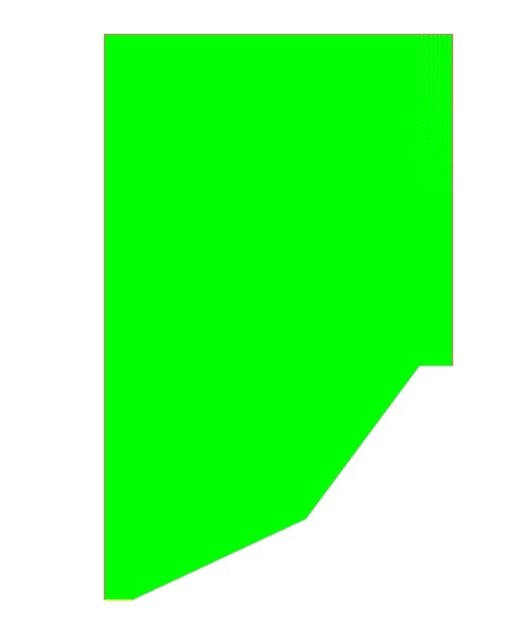
\includegraphics[width=0.9\linewidth]{images/mesh.jpg}
  \caption{ Computational Domain.}
  \label{fig:Mesh}
\end{minipage}%
\begin{minipage}{.5\textwidth}
  \centering
 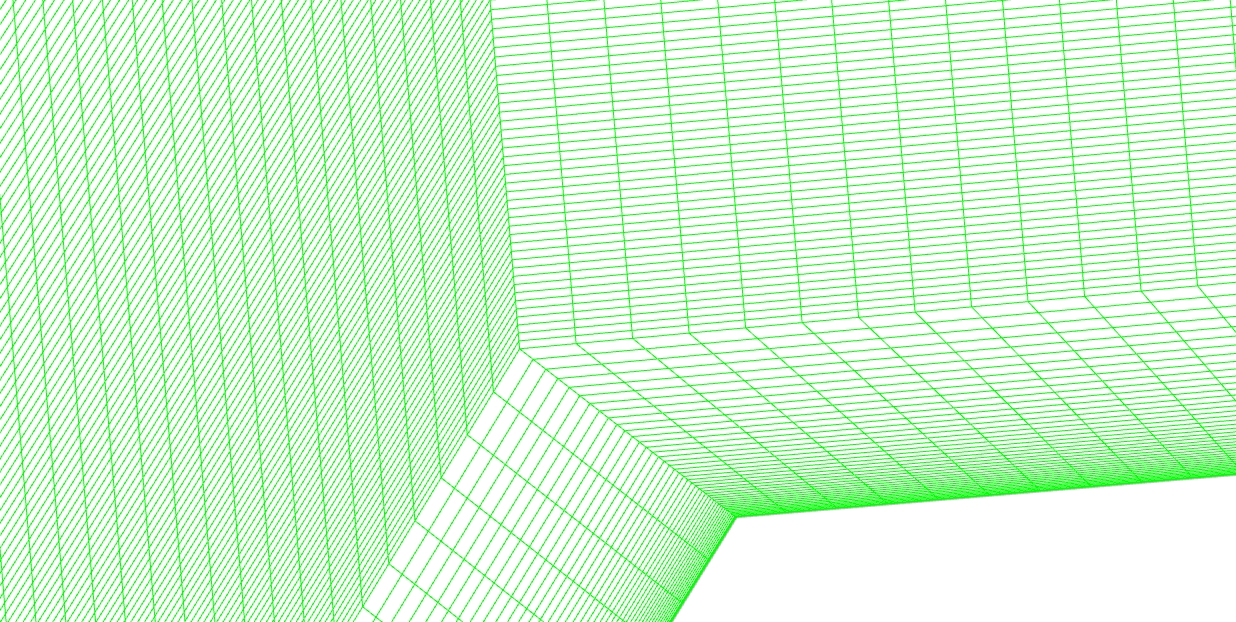
\includegraphics[width =0.9\linewidth]{images/boundary_layer.jpg}
  \caption{ Boundary layer mesh.}
  \label{fig:Boundarylayermesh.}
\end{minipage}
\end{figure}
\begin{figure}[ht]
\centering
  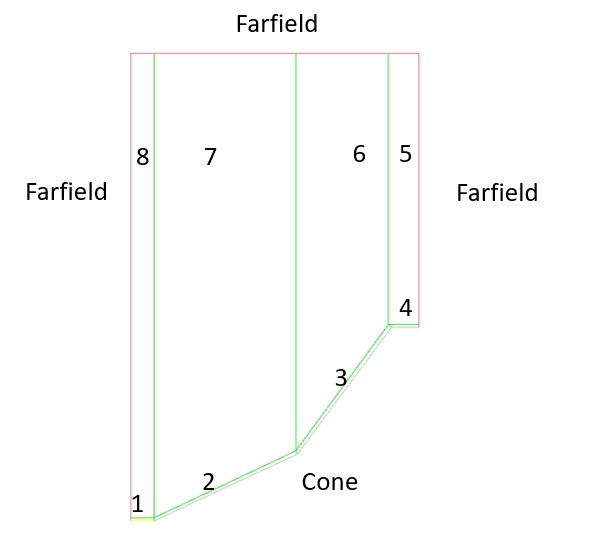
\includegraphics[width=0.55\linewidth]{images/mesh_zones.jpg}
  \caption{ Mesh Zones and Boundaries.}
  \label{fig:mesh_zones}
\end{figure}

The computational domain that is depicted in figure \ref{fig:Mesh} was generated using ICEM-CFD with a \( Y^+ \) maintained at 1-5, The first layer thickness was maintained at \(1 \mu m\), The mesh was divided into 8 zones and the mesh seeding is given in the table below, all the mesh seed size was maintained to 0.1 of the actual length, The mesh was completely a structured non uniform mesh with a total number of 2,83,000 cells which has been elaborated in Table \ref{fig:mesh_seeding}.

\begin{table}[h!]
\centering
 \begin{tabular}{||c c c||} 
 \hline
 Mesh Zone & Mesh seed (lxh) & Total Cells per zone \\ [0.5ex] 
 \hline\hline
 1 & 30 x 50 & 1500  \\
 2 & 200 x 50 & 10000  \\
 3 & 300 x 50 & 15000  \\
 4 & 100 x 50 & 5000   \\
 5 & 30 x 400 & 12000  \\
  6 & 200 x 400 & 80000  \\
  7 & 300 x 400 & 120000  \\
8 & 100 x 400 & 40000  \\
 \hline
 Total cells & &       283500\\
 \hline

 \end{tabular}
  \caption{ Mesh Zones and Mesh seeding .}
 \label{fig:mesh_seeding}
\end{table}

\begin{table}[h!]
\centering
 \begin{tabular}{||c c||} 
 \hline
Boundary & Boundary Definition  \\ [0.5ex] 
 \hline\hline
 Axis & Axis-symmetric Boundary \\
 Cone & Isothermal Wall (300 K)  \\
 Farfield & Pressure Far-Field   \\
 \hline
 \end{tabular}
    \caption{ Boundary and Boundary conditions.}
  \label{fig:bc_definition}
\end{table}


\begin{table}[h!]
\centering
 \begin{tabular}{||c c c||} 
 \hline
Symbol & Quantity & Flow conditions \\ [0.5ex] 
 \hline\hline
 \(M_{\infty}\) & Free-stream Mach Number & 10.38  \\
 \(H_{t\infty}\) & Free-stream Enthalpy (MJ/kg) & 3.96  \\
 \(U_{\infty}\) & Free-stream Velocity (m/s) & 2612  \\
 \(Re_{\infty}\) & Free-stream Reynolds Number (\(m^{-1}\))& 341.2 x \(10^3\) \\
 \(T_{\infty}\) & Free-stream Temperature (K)& 152.2  \\
 \(T_{wall}\) & Wall temperature (K) & 300  \\
 \(\rho_{\infty}\) & Free-stream Density (kg/\(m^3\))& 1.37 x \(10^-3\)  \\
 & Fluid & Ideal Gas  \\
 \hline
 \end{tabular}
  \caption{ Free-stream conditions [4]}
 \label{fig:freestream_conditions}
\end{table}

The wall boundary was defined as Isothermal wall and the far-field boundary condition was initiated with free-stream mach number and pressure. Since the body is a double cone geometry, the axis was defined as axis-symmetric boundary condition which is clearly depicted in Table \ref{fig:bc_definition}. Ideal gas is chosen and Reynolds Averaged Navier-Stokes was chosen as the main solver to solve the flow physics. 